%!TEX root = ../masters_thesis.tex

\chapter{Introduction} % (fold)
\label{cha:introduction}
\begin{large}
\begin{quoteit}
  Imagine there's no countries \\
  It isn't hard to do \\
  Nothing to kill or die for \\
  And no religion too \\
  Imagine all the people \\
  Living life in peace
\end{quoteit}
\end{large}
\hfill \textit{-- John Lennon, \emph{Imagine} (1971)}

John Lennon's song is an anthem for peace on Earth, not only for brotherhood of people, the end of materialism, but also for the end of countries. He connects the concept of a country to the nationalism that encourages people to fight and die for it. John Lennon wrote ``Imagine'' in the 1970s, in the midst of the Cold War between the capitalist and the socialist blocs, only 30 years after World War II and 50 years after World War I. Especially in Europe, this time would have probably not been described as ``peaceful''. And many, not just John Lennon, connected this lack of peace with the existence of national states divided by artificial borders.

Now, another 45 years later, the situation in Europe looks much different: most countries are united in a confederation of largely shared economies. While there are still countries with clearly defined borders, they are mostly of legal nature, but citizens of the European Union can travel freely within large parts of Europe. This concept is celebrated as a major achievement, but it is mostly forgotten that the concept of nations with solid borders has not been there 200 years ago. While traveling in those days was probably not as pleasant as it is today, Goethe at least did not need a passport when he traveled to Italy and back to Weimar. He also did not travel from the country ``Germany'' via ``Austria'' to ``Italy'', he instead crossed several duchies and principalities that do not exist any more.

% ==============================================================================
\section{Motivation} % (fold)
\label{sec:motivation}

What we might call ``our country'' today has changed a lot in the past. Hardly any of the current 193 member states of the United Nations are in the same borders as 100 years ago. Countries have evolved in time and space. Would it not be desireable to see this development? Would it not be interesting to have a map that shows the state of the world at any point in history? With this map we could see how our country looked like 100, 200 or even 1000 years ago. We could see how settlements became cities and principalities became national states. While there are many historical sources describing one point in history, may they be governmental bills, historical maps or diary entries of kings, there is no such thing as a comprehensive historical world atlas that lets you travel back in time and space and explore \emph{when} our country changed, \emph{where} it changed -- and most importantly \emph{why}? These is the question at heart of this thesis: How can the historical development of countries be visualized, for the benefit of a better understanding of how we became what we are today.

This is a very ambitious undertaking, given that countries have changed frequently. There are serious conceptual problems: How do we know how a country looked in 1600? If we find a historical map of this time, can we trust it? How certain can we be that the countries and their borders are correct? The next problem is that we are faced with contradictory histories of countries. There is not always \emph{one story} which is supported by all sides. There are contested territories, even today, whose ownership is unclear. There are ``places'', even today, which are not clearly a ``country'' because some might disagree. There is a great deal of uncertainty and disagreement in the body of history which this thesis addresses.

Finally, the state of the world cannot be visualized at any point in history just like this, since there is no freely available dataset. It is not just a visualization problem, it is a data problem. And to go even further: It is a data model problem, because it is not even straightforward to say what kind of information is actually necessary to show the history of countries. And if we found a data model and acquired some data, we would not want to manually write it into a database. The third goal for this thesis is to develop a well-designed user interface to edit the history of countries directly on the map.

\emph{TODO: figure new globe vs. old globe}

% section motivation (end)

% ==============================================================================
\newpage
\section{Problem Domain} % (fold)
\label{sec:problem_domain}

\begin{quoteit}
  All human action takes and makes place. \\
  The past is the set of places made by human action. \\
  History is a map of these places. \\
  The past thus exists not in time but in space.
\end{quoteit}
\hfill -- Philip J. Ethington in \cite[précis]{citeTakeMakePlace}

\emph{Time} and \emph{space} are everywhere. They are highly related to our lives and the objects we perceive. The temporal perception of the world is driven by events, may they be personal life events like a wedding or world events like the fall of the Berlin Wall. While a point in time can be described by a time stamp including a date, it is not always easy to scale and grasp. This is mainly because some temporal developments happen suddenly, like a natural disaster, and some happen very slowly throughout years, decades or even centuries, like climate change. Time is not tangible. For space, the situation is different, because it can be perceived as physically existing: a place is just there, we can go there and see it. Today, each point on this planet can be exactly described by a pair of geographic coordinates.

The combination of both concepts in one information system would allow to say how something has developed in time and space. \emph{Geographic Information Systems} (GIS) allow to manage and visualize data with a spatial relation to the Earth, mostly on a map. Most GIS answer two basic questions about an object: \emph{where} it is in relative or absolute location and \emph{what} it is -- an object with certain properties. As an example, a country can be expressed by a set of borders consisting of border points in geographic coordinates and by a name. However, most of the current GIS are limited to the spatial dimension. They cannot provide an answer to the question of \emph{when} a country was found or how its borders have developed in the previous fifty years. For that purpose \textbf{\emph{Historical Geographic Information Systems}} (HGIS) were developed. They extend general GIS with the dimension of time.

There exist several \emph{spatio-temporal data models} that deal with the temporal development of spatial objects. The straightforward approach immediately derives from the concept of historical maps: \emph{snapshots} are taken at certain points in time. They are maps that completely show the current state at this moment. Snapshots can immediately answer the question of what the world looked like at certain dates. However, they fail to answer the next question: what has changed since the last snapshot, when and why? Given two historical maps of Germany, one from 1871 after the formation of the German Empire and one from 1919 after the Treaty of Versailles -- how did it look like at the beginning of World War I in 1914? As shown in figure \ref{fig:snapshot_approach}, this is impossible to say, because there is no information about an arbitrary point in time between two snapshots. Also, if the map only shows Germany and its neighboring countries, what about Russia, Sub-Saharan Africa or South East Asia? For an interactive historical world atlas, the snapshot approach is neither suitable nor feasible, because it requires a whole new world map every time any country on Earth changes.

\begin{figure}[ht]
  \vspace{1em}
  \centering
  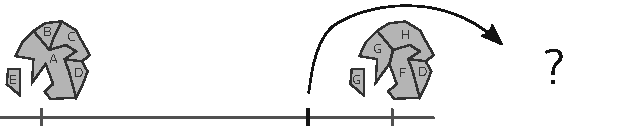
\includegraphics[width=0.9\textwidth]{graphics/introduction/snapshot_approach}
  \caption{The snapshot approach for modeling time and space}
  \label{fig:snapshot_approach}
\end{figure}


The key problem is that snapshots cannot express what has changed, because they do not store changes. This is the approach of another class of spatio-temporal data models: \emph{event-based} models. They store two things: one reference snapshot and a set of events that happen at a certain point in time and trigger changes on the map relative to the last event.

\begin{figure}[ht]
  \vspace{1em}
  \centering
  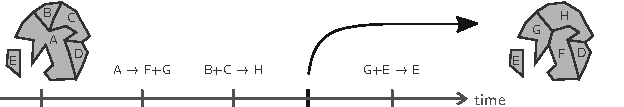
\includegraphics[width=0.9\textwidth]{graphics/introduction/event_based_approach}
  \caption{The event-based approach for modeling time and space}
  \label{fig:event_based_approach}
\end{figure}

Figure \ref{fig:event_based_approach} shows such an event-based approach: three changes are consecutively happening to the snapshot on the left. The question about the status of the world at an arbitrary point in time can be answered like this: it is the state of the reference map and each change of all events since that moment accumulated. In case of figure \ref{fig:event_based_approach}, country $A$ splits up into $F$ and $G$ and $B$ and $C$ unify to $H$. This approach is suitable for modeling a country's history, because each change to the state of a country was introduced by some historical event, may it be a declaration or a peace treaty.

% ------------------------------------------------------------------------------
\newpage
\paragraph{Research Questions} % (fold)
\label{par:research_questions}

The goal of this thesis is to lay a theoretical foundation for a HGIS that deals with the development of countries in time and space. The domain is limited to countries, their names and borders as well as historical events that change them. In addition, the model is to be developed in HistoGlobe, an open-source web-based application that aims to visualize the course of history. It should provide a well-designed user interface for editing historical data about countries allowing the user to directly manipulate the countries on the map. There are three research questions to be answered throughout the thesis:

\begin{enumerate}
  \item What type of historical changes can happen in the development of countries in time and space?
  \item How can these changes be
  \begin{enumerate}
    \item modeled in an information system?
    \item edited by humans in a user interface?
  \end{enumerate}
  \item How can the model handle uncertainty and disagreement in history?
\end{enumerate}

% paragraph research_questions (end)

% ==============================================================================
\section{Overview} % (fold)
\label{sec:overview}

The remaining part of this Master's thesis is structured in four chapters. The second chapter introduces the basic concepts of the problem domain: First of all the surprisingly difficult concept of a \emph{country} is introduced in section \ref{sec:countries}. Afterwards the term \emph{Historical Geographic Information Systems} is clarified in section \ref{sec:historical_geographic_information_systems}, followed by state of the art of \emph{spatio-temporal data models}  in section \ref{sec:spatio_temporal_data_models}. Finally, section \ref{sec:histoglobe} presents \emph{HistoGlobe}, the application that the work of this thesis is developed in.

Chapter 3 is the main part of this thesis. It describes the Human-Centered Design process to answer the first two research questions. The \emph{Hivent model} in section \ref{sec:hivent_model} introduces a set of five \emph{Hivent operations} that are able to model all possible changes to the development of countries in time and space. The next section \ref{sec:editing_hivent_data} presents approaches to modify data in the Hivent model using \emph{edit operations}, a different set of operations that is well-understood by humans. The iterative design process of the user interface is illustrated in section \ref{sec:user_interface_design_process}. The chapter closes in \ref{sec:implementation} with an insight into the implementation of the data model and the user interface in the HistoGlobe application.

The fourth chapter tackles the last research question: how to deal with uncertain historical data? The model and the implementation of chapter 3 are evaluated in section \ref{sec:evaluation}. The shortcomings of the initial model are addressed in additional approaches that are developed to handle some aspects of uncertainty regarding the historical development of countries. The designed extensions are presented in section \ref{sec:modelling_uncertainty}.

In the last chapter 5 the thesis summarizes the work by answering the research questions. The work finishes with an overview about remaining questions, identified problems and possible approaches to solutions that are subject to future work on this topic.

% section overview (end)

% ==============================================================================

% chapter introduction (end)